\documentclass[a4paper,11pt]{article}
\usepackage[margin=2cm]{geometry}
\usepackage{anysize}
\usepackage[pdftex]{graphicx}
\usepackage{subfigure}
\usepackage{url}
\usepackage{listings}
\usepackage{textcomp}
\usepackage{wrapfig}
\usepackage{fixltx2e}
\usepackage{color}
\usepackage{fancyhdr}
\usepackage[nodayofweek]{datetime}
\usepackage[small,compact]{titlesec}
\usepackage[pdfborder=0]{hyperref}
\longdate

\definecolor{dkgreen}{rgb}{0,0.6,0}
\definecolor{gray}{rgb}{0.5,0.5,0.5}
\definecolor{mauve}{rgb}{0.58,0,0.82}
\definecolor{light-gray}{gray}{0.95}

\lstset{ %
  language=Java,                % the language of the code
  basicstyle=\footnotesize,           % the size of the fonts that are used for the code
  numbers=left,                   % where to put the line-numbers
  numberstyle=\tiny\color{gray},  % the style that is used for the line-numbers
  backgroundcolor=\color{light-gray},
  stepnumber=1,                   % the step between two line-numbers. If it's 1, each line 
                                  % will be numbered
  numbersep=5pt,                  % how far the line-numbers are from the code
  showspaces=false,               % show spaces adding particular underscores
  showstringspaces=false,         % underline spaces within strings
  showtabs=false,                 % show tabs within strings adding particular underscores
  tabsize=2,                      % sets default tabsize to 2 spaces
  captionpos=b,                   % sets the caption-position to bottom
  breaklines=true,                % sets automatic line breaking
  breakatwhitespace=false,        % sets if automatic breaks should only happen at whitespace
  title=\lstname,                   % show the filename of files included with \lstinputlisting;
                                  % also try caption instead of title
  keywordstyle=\color{blue},          % keyword style
  commentstyle=\color{dkgreen},       % comment style
  stringstyle=\color{mauve},         % string literal style
  escapeinside={\%*}{*)},            % if you want to add a comment within your code
}

\setlength{\parskip}{10pt} 
\setlength\parindent{0pt}
\pagestyle{fancyplain}
\fancyhf{}
\lhead{\fancyplain{}{M.Sc.\ Group Project Report}}
\rhead{\fancyplain{}{\today}}
\cfoot{\fancyplain{}{\thepage}}


\title{Twitter for traffic\\\Large{--- Final Report ---}}
\author{Porfyrios Vasileiou, Marianna Polatoglou, Afxentios Hadjiminas,\\
        Panagiotis Tsirigotis, Hanguang Zhou, John Flanagan.\\
       \{pv311, mp1911, ah2411, pt1111, hz511, jf311.\}@doc.ic.ac.uk\\ \\
       \small{Supervisors: Dr.\ Emil Lupu, Dr.\ Alessandra Russo, Dr.\ Luke Dickens}\\
       \small{Course: CO533, Imperial College London}
}

%Report details http://www.doc.ic.ac.uk/~cristic/teaching/MScGroupProj/

\begin{document}
\maketitle
\pagebreak
\tableofcontents
\pagebreak
\section{Introduction}
	City planners have been struggling to acquire real-time data on traffic
conditions. This data is especially important with incidents which may
translate into traffic disruptions on an already over capacity road network.
Cities have experimented with traffic cameras, dynamic traffic light control
and more traditionally traffic based radio stations.

Internet connected mobile phones and micro-blogging platforms like Twitter have
been providing researchers with a vast and interesting source of real-world
data. This data has been used to analyse trends, identify concepts and to
augment traditional curated data providing a level of social knowledge to the
topic.

Twitter for traffic aims to take these concepts to provide the mobile user with
an application for assessing traffic disruptions as they evolve for London
city. To provide this insight, the application will present the user with
curated traffic disruptions augmented with social knowledge of the event
harvested from a social network.  In addition to this curated list of traffic
disruptions, the concept of identifying emerging disruptions from this social
data will be explored, with the aim of identifying clusters of disruption
reports to discover new disruption events.

To promote the of reporting the traffic conditions on a social network, it will
also be necessary to provide a fast, simple and descriptive mechanism for the
user to manually contribute their observations.

There are a number of interesting challenges the comprise this task. Initially
we must identify tweets from Twitter that discuss road traffic. For these
traffic tweets to be of value we must be able to infer some geographic location
for each tweet, a small percentage of tweets actually contain a geographic
    location so other methods must be explored. To identify events from tweets
    alone, we must investigate geographic clusters of tweets which discuss
    traffic. There are a number of problems in detecting valid traffic
    effecting events, these include sufficient data, timeliness of the tweets
    and  ‘normal’ levels of background chatter.

    From the onset there are many unknowns relating to the data analysis,
    including the quantity of traffic related messages and quality of the
    content. Aspects of this project include data mining, social network
    analysis, mobile application development, document classification and
    geographical information systems.


\pagebreak
\section{Specifications}
	\subsection{Server}

\begin{center}
\begin{tabular}{ | p{9cm} | c | c | p{1.8cm} | }
\hline
\multicolumn{4}{|c|}{\textbf{Server Application}} \\ \hline
\textbf{Feature} & \textbf{Priority} & \textbf{Feasibility} & \textbf{Due date}
\\ \hline
\textbf{Store disruptions from TfL} \newline
Create a geographic database of live events from TfL. Evolve these database events with data from the feed, in order to have a current representation of the event. & 1 & 3 & Week 2 \\ \hline
\textbf{Store and categorise social data} \newline
For tweets with an explicit location, store them in a geographical database
table. And those tweets without this explicit information store them separately for later
analysis. & 2 & 2 & Week 2 \\ \hline
\textbf{Process mobile client reports} \newline
Take twitter messages reported from the mobile client and process these in a
separate pipeline. & 3 & 2 & Week 6 \\ \hline
\textbf{Classify tweets from Twitter with a simple classifier} \newline
Train a document classifier using a manually labeled training set to 
identify traffic related tweets. & 4 & 5 & Week 5 \\ \hline \hline
\textbf{Identify traffic disruptions from Twitter} \newline
Inspect incoming traffic tweets and determine new non-TfL disruptions from
those. & 5 & 5 & Week 5 \\ \hline
\textbf{Geocoding of messages without explicit locations} \newline
Resolve geographic locations extracted from the message context. & 6 & 7 & Week 6 \\ \hline
\textbf{Enhance classification and clustering algorithms} \newline
From insight and data gained from initial classification and clustering
techniques, attempt to improve the accuracy of the results. & 7 & 9 & Week 7 \\ \hline
\textbf{Store traffic cameras by geolocation(New)}\newline
Store a list of public traffic cameras in the database by their geographic
location. When returning traffic disruptions in the vicinity of a camera,
attach a link to the most relevant camera. &  8 &  4 & Week 7 \\ \hline
\multicolumn{4}{|c|}{Minimum specifications for the server application are
features including and below priority 4.} \\ \hline
\end{tabular}
\end{center}

\subsection{Client}

\begin{center}
\begin{tabular}{ | p{9cm} | c | c | p{1.8cm} | }
\hline
\multicolumn{4}{|c|}{\textbf{Mobile Application}} \\ \hline
\textbf{Feature} & \textbf{Priority} & \textbf{Feasibility} & \textbf{Due date} \\ \hline
\textbf{Report events}\newline
Report traffic disruptions through the mobile application on Twitter. & 1 & 2 & Week 3 \\ \hline
\textbf{Present a list of classified and grouped tweets}\newline
Present to the user tweets identified as describing a traffic disruption,
clustered around an event. & 2 & 4 & Week 6 \\ \hline
\textbf{Show local disruption map}\newline
Show positions of known disruptions on a map. Enable the user to click on an event for further information. & 3 & 5 & Week 6 \\ \hline
\textbf{Stored Routes}\newline
Find and show disruptions for user defined stored routes. & 4 & 7 & Week 7 \\ \hline \hline
\textbf{Present tweets on the map}\newline 
Display high ranked tweets on the map.& 6 & 7 & Week 6 \\ \hline 
\textbf{Present traffic camera for events}\newline
If a traffic event occurs in the vicinity of a traffic camera, present the user
with a camera icon. If they click on the icon they are presented with a live
view of the event. &  8 & 4 & Week 7 \\ \hline
\multicolumn{4}{|c|}{Minimum specifications for the mobile application are
features including and below priority 3.} \\ \hline
\end{tabular}
\end{center}


\pagebreak
\section{Conceptual Design}
	\input{conceptual_design/conceptual_design}

\pagebreak
\section{Design}
	
\subsection{System overview}
	\begin{center}
	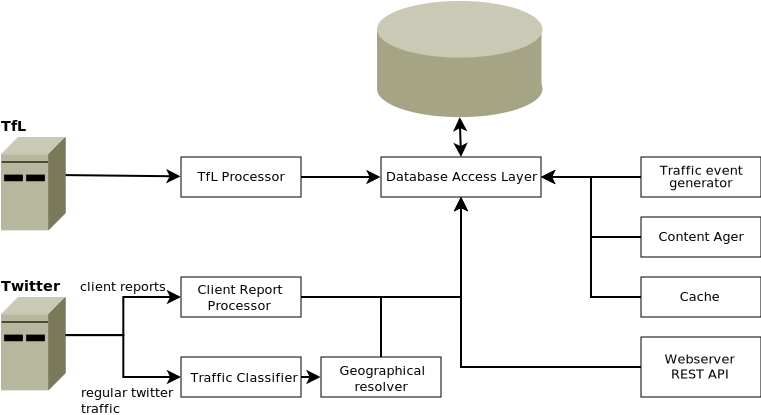
\includegraphics[scale=0.37]{images/high_level_system_arch.pdf}
	\end{center}
\subsection{Server}
  \begin{figure}[htb]
\centering
\includegraphics[width=1\textwidth]{images/design/server/server.pdf}
\caption{Server Design}
\label{fig:server_design}
\end{figure}

\subsubsection{Data acquisition}
The sources that we collect data from are Transport for London (TfL) and Twitter.

\paragraph{1. TfL Disruption Events}
The TfL website provides different types of data feeds that can be used to obtain information relevant to traffic. 
One of the TfL data feeds we use is the "live traffic disruptions". This provides information about traffic disruption events in the area of London. This information contains details about the severity of the event, the type (e.g. road works, signal failure, accident), the location and an estimated time for the event's end.

\paragraph{2. TfL Traffic Cameras}
To provide a more complete view around the area of the event we also store the "live traffic camera images" feed from TfL. This provides URLs to pictures taken by traffic cameras within the last 15 minutes as well as the location of the camera and the timestamp when the picture was taken.

\paragraph{3. Twitter}
For Twitter we defined the area around London that we are interested to collect tweets from. In addition to this, we used a search query with the words that we want the results from Twitter to contain. This query is consisted of words chosen after experimentation.

\subsubsection{Data analysis}
\paragraph{1. TfL Feeds Processing}
The TfL feeds we used for the application are returned as XML files. Using the minidom python library, we were able to parse them. Because a TfL traffic event's position is returned as a point in British national grid coordinates, we first transform them to longitude and latitude coordinates before storing them in the database. This is done using a python module that implements the algorithm given in the ordnance survey guide.\cite{website:grid2lonlat_alg} \cite{website:grid2lonlat_impl}

\paragraph{2. Twitter Processing}
In contrast to the TfL, the Twitter data are returned in a JSON format. For this reason, we used the python-twitter API which saves the JSON information into classes and variables that can then be easily accessed. Before storing the tweets to the database each of them passes through a processing pipeline.

First, the username of the person who sent the tweet is checked to find out if he is in the blacklist. The blacklist is a txt file we have in the server which can contain different usernames for twitter accounts from which we do not want to store tweets. The reason for this is that we can use this blacklist for traffic (or other) bots so that we only have real persons' tweets in the database. Then, we use the classifier to decide if the tweet's text is about traffic or not. The process of classification is described in the Classification section. After classifing a tweet as traffic, we use a regex to find any streets or roads in its text. Finally, before storing the tweet we check a list of words that we have in a txt file to determine if they are included in the message. This is implemented for a profanity filter.

\subparagraph{2.1. Classification}
A big and crucial part of the project was the data analysis. Specifically for the needs of the project a sub category of the data analysis, which is called text classification, has been implemented. The text classification was necessary because the project is required the tracking of the traffic-about tweets and their presentation in the application. Moreover, the identification of the disruptions through the clustering of the tweets, is strongly depended with the recognition of the tweets as traffic or as non traffic. 

Text classification is a way to categorize documents or pieces of text. By examining the way the words are being used in a piece of text, classifiers can decide, after the training, what class label to assign to it. A binary classifier decides between two labels, such as traffic or non-traffic. The text can either be one label or the other, but not both, whereas a multi-label classifier can assign one or more labels to a piece of text. 

Two approaches for the automatic document classification exist: the supervised document classification and the unsupervised classification (clustering). The supervised classification requires a training data from the humans in order to gain the “knowledge” of the classification. The clustering doesn’t require human to have the foreknowledge of the classes, and mainly using some clustering algorithm to classify a text. The team decided to adopt the supervised classification because it’s a more stable technique and it can be used as soon as the classifier is been trained. On the other hand, the unsupervised classification has to start somewhere, and its algorithms try in iterative ways to reach a stable configuration that makes sense. Therefore it may require a large amount of time to reach this configuration, halting the rest development pipeline of the project. That’s because the classified data is required from other parts of the project. Additionally, the results of the unsupervised classification vary widely and may be completely off if the first steps are wrong.

Classification works by learning from labelled feature sets, or training data, to later classify an unlabelled text, or a feature set. A feature set is basically a key-value mapping of feature names to feature values. In the case of text classification, the feature names are usually words or blocks of words, and the values are all True. As the texts may have unknown words, and the number of possible words may be very large, words that don't occur in the text are omitted, instead of including them in a feature set with the value False.

For the project it was essential to classify the tweets that the Search API was fetching, as traffic or as non-traffic. The non-traffic tweets are being rejected while the tweets about traffic are being stored in the database, in order to be correlated with the current disruption and then presented to the application. For this purpose several classification techniques have been implemented and tested. To be more specific, the team has investigated the classification of the tweets with the methods Support Vector Machines and Naive Bayes. 

Those two algorithms have been selected cause of a number of reasons. Firstly, Naive Bayes train very quickly since it requires only a single pass on the data   to compute the normal probability density function. It also requires little storage space during both the training and classification stages: the strict minimum is the memory needed to store the prior and conditional probabilities. Additionally Naive Bayes is very transparent, as it is easily grasped by users and it provides a discrete probability for each tweet helping the ranking of the tweets. Naive Bayes is considered to have high bias, because it assumes that the dataset under consideration can be summarized by a single probability distribution and that this model is sufficient to discriminate between classes. This high bias usually generates simple, highly constrained models. On the other hand, SVM is considered to be one of the most accurate classifier when dealing with multidimensions and continuous features. However for the SVM, a large sample size is required in order to achieve its maximum prediction accuracy whereas Naïve Bayes may need a relatively small dataset.

\textbf{Naive Bayes}

Given a set of objects, each of which belongs to a known class, and each of which has a known vector of variables, the aim is to construct a rule which will allow the assigning of future objects to a class, given only the vectors of variables describing the future objects. Problems of this kind, called problems of supervised classification, are ubiquitous, and many methods for constructing such rules have been developed. One very important method is the Naive Bayes Reasoning. This is a well- established Bayesian method primarily formulated for performing classification tasks. Given its simplicity Naive Bayes models are effective classification tools that are easy to use and interpret. Naive Bayes is particularly appropriate when the dimensionality of the independent space. For the reasons given above, Naive Bayes can often outperform other more sophisticated classification methods. A variety of methods exist for modelling the conditional distributions of the inputs including normal, lognormal, gamma, and Poisson. 

This classifier has been created using the Bag of Words model and the NLTK suites of libraries. NLTK is the Natural Language Toolkit, a comprehensive Python library for natural language processing and text analytics. The group decided to use the Natural Language Toolkit because of its simplicity, consistency, extensibility and its modularity. Additionally some of the members had already experience with it and they were aware of its efficient and its good classification results. Furthermore, it was decided the usage of the Bag of Words feature extraction. Text feature extraction is the process of transforming what is essentially a list of words into a feature set that is usable by a classifier. The NLTK Naive Bayes classifier expects dictionary style feature sets, so the text should be transformed into a dictionary. The Bag of Words model is a well-known method for representing documents, which ignores the word orders. It constructs a word dictionary from all the words of an instance where every word gets the value True. An instance is a single feature set. It represents a single occurrence of a combination of features. A labelled feature set is in fact an instance with a known class label that we can use for training or evaluation.

As it has been mentioned before, for the training of the classifier it’s required a labelled data. To accomplish that, a simple script was created. This script was being executed on a temporary table on the database which was containing raw, unlabelled, tweets. During the execution it was presenting random tweets from this table and the user was able to press four buttons in order to label the tweets as traffic (personalized tweets about traffic), non-traffic, unclear and bot (tweets about traffic from official sites). After the gathering of a big amount of traffic-about tweets, the table in which the labelled tweets were being stored was used to train the classifier. However, before this data was used to train the classifier, a several linguistic normalization has been applied on the labelled text.  More details for the normalization will be described in a next section.

\textbf{Support Vector Machines}

The second supervised learning method that was integrated and tested is the Support Vector Machines (SVM). This is a method that performs regression and classification tasks by constructing nonlinear decision boundaries.

In this project PyML\cite{website:pyml} was used to implement SVM
classification. The results of this algorithm did not show much improvement
compared to Naive Bayes classification. Also the library seems to be at an
early stage, and is still quite buggy. This makes it more difficult to use
and it is not that stable to be included in the product. Since the accuracy
does not change, the use of Naive Bayes was decided by the group.

\textbf{Normalization}

For both of the above methods a separate class has been created to be used for the tweets normalization. Normalization is the way to eliminate the low information features. Eliminating low information features gives to the model clarity by removing noisy data. Additionally it reduces the possibility to get over-fitting. By using the higher information features, the performance is increasing while the size of the model is decreasing, which results in less memory usage along with faster training and classification. This normalization was being applied on the labelled tweets before the classifier training and is continue being applied on the newly fetched tweets as well. Using this pre-processing on the tweets the accuracy of the classifier has been increased. On the following paragraphs we will present the normalization techniques which have been adopted. 

The first step was to convert the current links to a more readable way. This has been done by using a regular expression to recognize the link. After that the domain is being extracted from the url and it replaces the link itself. The next step is to replace the emoticons with a global name so they will not be deleted during the punctuation removal. That’s important because the emoticons offer useful information during the classification. For this purpose, the team has integrated a script which is responsible to find those emoticons, assign them to a group of emoticons and replace them with the name of the group. Four groups of emoticons have been created: Happy, Sad, Very Happy, Very Sad. The next step is to remove the punctuations. The team has accomplished that by creating a regular expression which represents all the possible punctuations. 

After the above linguistic transformations, the tweets are being tokenized into words. Then the unnecessary special words, like the usernames, are being removed from the tweets. Subsequently, lemmatization is being applied on the tokenized data by removing and replacing word suffixes to arrive at a common root form of the word in order to group up the common words. This method has been chosen over the stemming, because lemma is a canonical set of words, instead of the stem which in many cases is not a real world. Afterwards several stopwords have been ignored from the tweet during the classification. However, because of the natural of the tweets of being an unstructured language, the accuracy of the classifier has dropped radically. Therefore the team decided not to use the stopwords as part of the normalization. The last but not least step of the text normalization is the tracking of the bigrams collocations from the tweets. Because the bigrams are less common than most individual words, including them in the Bag of Words increases the classifier accuracy.

\textbf{Soundex}
When people are typing tweets, there are some spelling mistakes or abbreviations in them. It is difficult for server to understand the meaning of those sentences with spelling mistakes or abbreviations.This project introduce Soundex algorithm which is a phonetic algorithm for indexing names by sound, as pronounced in English. Its goal is for homophones to be encoded to the same representation so that they can be matched despite minor differences in spelling. The algorithm mainly encodes consonants; a vowel will not be encoded unless it is the first letter. That means a wrong street name will probably matches the right street name if the first letter in the street name is not typed wrongly.
In project, a 'geolookup' table which stores street address is created for looking up geolocation. When a tweet doesn't have geolocation, it will be parsed to extract street address which is used to search corresponding geolocation in 'geolookup' table. However, some addresses cannot find geolocation because there is spelling mistakes or abbreviations in it. We split street address into independent words and remove white-spaces inside. Then we encode those words using Soundex algorithm to get results and combine them into a string. This string created by Soundex algorithm is compared with other Soundex strings which is converted from street addresses in 'geolookup' table. This algorithm improves the ratio of street address matching.



\subsubsection{Storage}
For the storage of data we use a PostgreSQL database. This decision was made because PostgreSQL is one of the most stable open source database management systems. Due to the large amount of database queries, we needed to use an efficient way to store and analyze the information we acquired from the TfL feeds and Twitter. For this reason, we decided to use a Geographic Information System called PostGIS, which is a spatial database extension for PostgreSQL. This allowed us to store geolocations (longitude and latitude) as points.

With the use of PostGIS, queries to the database became easier and more efficient. The use of functions provided by PostGIS, such as \emph{ST\_DWithin} to find all points around a route or a point within a radius, or \emph{ST\_Distance} to find the distance between two points, made all queries simpler. In addition, the main advantage of PostGIS is that it uses generalized search trees (GiST) to index the geometries. 

A GiST like a B-tree uses key-pointer pairs. The difference with B-trees is that a GiST key is a user-defined data type. This allows different types of operations, rather than simple comparisons, such as nearest-neighbor searches and statistical approximations over large data sets. In PostGIS, the GiST is used for spatial indexing by allowing the index to use a bounding box for each geometry (e.g. line) instead of storing the whole geometry in it. Therefore, with bounding box comparison, instead of comparing geometries, functions such as ST\_DWithin are made more efficient. \cite{website:postgis_stdwithin}

For the project we used the following tables:
\begin{itemize}
\item Tables used by the final application
  \begin{itemize}
  \item \emph{tfl}: The current tfl disruption events
  \item \emph{archive}: To store old tfl disruption events for further analysis
  \item \emph{tflcameras}: The current camera pictures' url
  \item \emph{tweets}: To store the traffic tweets acquired from twitter
  \item \emph{geolookup}: Used to store addresses with their Soundex value and their geolocation which is acquired from Google Maps
  \item \emph{tweets\_metrics}: Used to store different types of metrics for the tweets
  \end{itemize}
\item Tables used to train the classifier
  \begin{itemize}
  \item \emph{labelled\_tweets}: To store manually labelled tweets as traffic or non-traffic
  \item \emph{stop\_words}: Words that can be removed before data analysis
  \end{itemize}
\item Tables used by PostGIS
  \begin{itemize}
  \item \emph{geography\_columns}: This is a view that shows all the columns of the database that use geography points
  \item \emph{spatial\_ref\_sys}: A list of spatial reference systems and details to transform between them
  \end{itemize}
\end{itemize}

\subsubsection{Interface}

Before the server implementation, the creation of a mock server api was essential. This 
provided us with the ability to seperate the work on the application and server design from the very 
beginning of the project. At this stage, the rest endpoints had to be defined in order to agree on the 
data format that was transferred between the server and the client. The next thing was creating mocked 
JSON data for responding to the requests. Such data included fixed sets of disruptions, tweets and 
cameras.

The server consists of several threads. Three of these threads are used to collect the data feeds from TfL and messages from Twitter, as described in a previous section. Another thread is used by the Representational State Transfer (REST) server to receive and respond to mobile client requests. The reason for the implementation of the different threads is to achieve a fault resilient server. If one of these threads stops working because of an unexpected error, the remaining threads can continue to work unaffected. Furthermore, each thread stores a log to a file about its actions and errors it has encountered, which makes debugging simpler.

The REST server can receive GET or POST requests from the mobile client. If the request was not in the correct format then the server returns a bad request (Error 400). The response to these requests is a JSON file. 

The server and the mock server can run at the same time on different ports. Each request uses a URL that has the version written in it. This achieves old version compatibility, as the server can continue to support previous client versions. In the following requests the version is named 0.2:
\begin{itemize}
\item \emph{GET} \url{/t4t/0.2/disruptions} \\
Parameters: \emph{longitute, latitude, radius, closestcam (optional)} \\
Description: A request that returns all current disruptions in an area defined by a point (longitude and latitude) and a radius. There is also an option to return only the closest camera for each request.

\item \emph{GET} \url{/t4t/0.2/disruptions} \\
Parameters: \emph{topleftlat, topleftlong, bottomrightlat, bottomrightlong, closestcam (optional)} \\
Description: A request that returns all current disruptions in an area defined by 2 points that are the 2 opposite corners of a rectangle. There is also an option to return only the closest camera for each request.

\item \emph{GET} \url{/t4t/0.2/disruptions/route} \\
Parameters: \emph{JSON encoded list points on a route} \\
Description: A request that posts a json file of points on a route that will return all disruptions around it.

\item \emph{GET} \url{/t4t/0.2/tweets} \\
Parameters: \emph{disruptionID, filter (optional)} \\
Description: A request that returns all tweets that are around a disruption event. There is also an option to use the profanity filter for the tweets that are returned.

\item \emph{GET} \url{/t4t/0.2/tweets} \\
Parameters: \emph{longitute, latitude, radius, filter (optional)} \\
Description: A request that returns all tweets in a area defined by a point (longitude and latitude) and a radius. There is also an option to use the profanity filter for the tweets that are returned.

\item \emph{GET} \url{/t4t/0.2/cameras} \\
Parameters: \emph{disruptionID, closestcam (optional)} \\
Description: A request that returns all cameras that are around a disruption event. These requests have an option to return only the closest camera.
\item \emph{GET} \url{/t4t/0.2/cameras} \\
Parameters: \emph{longitute, latitude, radius, closestcam (optional)} \\
Description: A request that returns all cameras in a area defined by a point (longitude and latitude) and a radius. These requests have an option to return only the closest camera.

\end{itemize}


\subsection{Client}
  The Google Android operating system was chosen as the client platform. This
decision was based primarily on two factors, firstly that the teams mobile
development experience was mainly with Android and additionally the
availability of development hardware for the duration of the project.

As a part of our white-boarding meetings, we developed a high level idea of the
functionality required by the client interface this can be seen in
Figure~\ref{fig:system_components}.

To create a structure for the client the team explored a number of low fidelity
user interface options. The agreed upon interface was used as a basis to create
an architecture for the project. The identified components and their
communications are described in Figure~\ref{fig:client_design}.

\begin{figure}[htb]
\centering
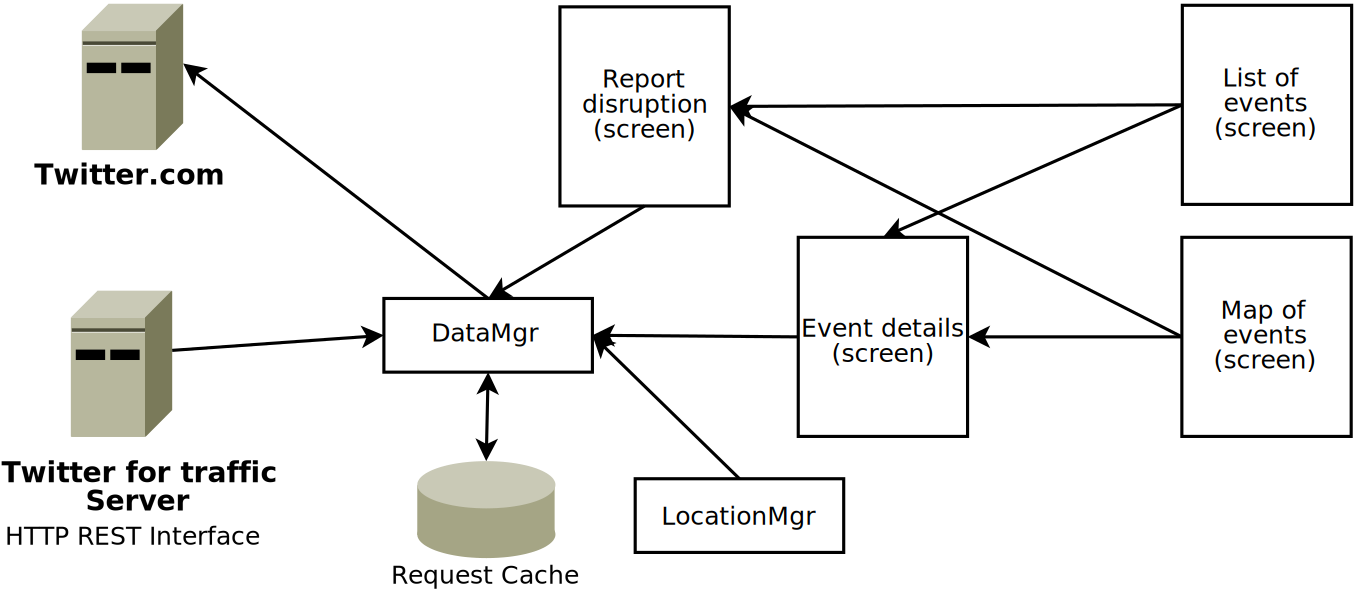
\includegraphics[width=0.9\textwidth]{images/design/client/client_high_level_layout.pdf}
\caption{High level client design}
\label{fig:client_design}
\end{figure}


\subsubsection{Server interface}
As previously discussed in this document, a ‘mock’ server was created to
parallelise efforts and to verify the REST endpoints. This tool proved very
useful in the development of the client application, particularly with verbose
logging on the server side when debugging connection issues.

The interaction with the server is encapsulated in the \emph{DataMgr} class.
This class returns lists of the relevant object types to the requester. The
interface for this class can be seen in Listing \ref{datamgrinterface}.

\lstset{caption={DataMgr.class public interface},label=datamgrinterface}

\begin{lstlisting}
public DataMgr(Context context);
public List<EventItem> requestEvents();
public List<TweetItem> requestTweets(String eventID);
public List<EventItem> requestRouteEvents(Route route);
\end{lstlisting}

\subsubsection{Request caching}
Modern mobile data networks have increased data-rates to an incredible level
over the last number of years, it is not uncommon now to see providers offering
speeds of 7.2 Mbps. But these types of networks also tend to incur large
latencies, for an initial TCP request from mobile handset round trip times of
up to one second are not unheard of.

As a mechanism to make the application feel more responsive to the user, the
application caches the response from the previous request. This cached response
is displayed if delays or issues occur but once fresh data becomes available
the screen is populated with this data. Most typically delays occur in
acquiring a geographical lock, as we require a current geographical location to
make an event request. Or being unable to contact the server due to
connectivity issues.

\subsubsection{Twitter interface}
\subsubsection{Home route functionality}
\subsubsection{User interface}




\pagebreak
\section{Methodology}
	To begin identifying an appropriate development methodology, it is necessary to understand the project requirements. The project requirements and features are determined over a number of meetings with the primary stakeholders. 

At this point, the development methodology can be determined. Since we are looking for iterative and incremental development, Agile Software Development Methodology will be followed. This also enables time-boxed iterative approach. Agile methods are focused on different aspects of the software development life cycle. Two of the most well known agile methodologies are Scrum and XP.

Scrum is an agile project management technique that focuses more on the management of software development projects. The product is completed in a series of one to four week iterations, or sprints. Before each sprint, a planning meeting is held to define which features will be implemented during that sprint. Similarly, XP (Extreme Programming) is an agile methodology which is designed for small, co-located teams aiming to get quality and productivity as high as possible. It does this through the use of rich, short, informal communication paths with emphasis on skill, discipline, and understanding at the personal level, minimizing all intermediate work products.

As this is a college project and tight time constraints apply, it is quite
difficult to follow a particular methodology. Scrum focuses on the management
side of the project whereas XP focuses more on the actual programming
practices. It is more preferable if various elements from both methodologies
can be used, since they address different areas and complement each other.

Therefore, it was decided to focus on managing the software project using the scrum
approach and adopt characteristics that suit the project. Weekly meetings are planned to organise the division
of work and for the team to get up to speed with all the tasks in progress and recently
completed. An agenda for each meeting is stored in an online document, that
each team member may add to. 

To encourage a more agile development the online collaboration tool
Trello is used. This tool gives access to a visual board that displays the
on going tasks. These tasks are represented as cards with labels and priorities. 
Trello is very similar in concept to the scrum board, as shown in fig 2.

\begin{figure}[here]
\begin{minipage}{\textwidth}  
\begin{center}
\includegraphics[width=0.95\textwidth]{images/scrumboard.jpg}
\end{center}
\vspace{-20pt}
\caption[Caption for LOF]{Scrum Board and Trello\footnotemark}
\end{minipage} 
\end{figure}
\footnotetext{Left: Drew Stephens \url{flickr.com/photos/dinomite/3695570625}, Right: \copyright \url{Trello.com}}

It was agreed that adopting techniques from XP would help to
improve the development process. Pair programming is one of those techniques the team would strive to adopt.
Two programmers work alongside on the same code and together they develop a single feature. Constant refactoring is another key practice to be adopted. Any
time the two find a section of code that appears hard to understand or overly
complex, they are to revise it, constantly simplifying and improving it. Furthermore, a test driven approach will be taken during this development.
However because of the nature of the project being partly research based and
the results being quite subjective, it is difficult to test effectively. Hence,
the development of the mobile application will be test-driven whereas for the
server development it will not be possible to follow test driven approach so strictly\cite{Cockburn}. These techniques improve the code quality and team focus.

For the division of work amongst the team, more flexibility will be achieved by maximising the use of the members previous experience. A division has been decided where two members of the team will focus on the mobile application, three on the server side and the final person will move between these tasks as necessary. A team leader is also designated with the aim of coordinating the two development efforts.  

To achieve parallel development, the server API will be agreed and mocked-up returning a static data set. That way, those developing the mobile application can work independently from those working on the server.

The mobile application is the only user facing aspect of the project. The user interface will be agreed using a series of LoFi (pen and paper) concepts, to prove that they provide the required features in a user friendly manner.



\pagebreak
\section{Group Work}
	\subsection{Team Structure}
Project management is a necessary part of group  project. Trello is a easy tool for us to plan this project well. We set four statements for anything we want to do: 'To Do', 'Started', 'Review' and 'Done'. At the same time, six labels are built with different colours to identify their kinds of tasks: 'Data', 'Documentation', 'Server', 'Android App', 'Text Analysis' and 'Meeting Prep'. All tasks will be discussed at week meeting and assigned to 'To Do' list. When team member who is responsible for the task will drag this task card to 'Started' list to inform others that this task is being done. After this task has been finished, team member will move this task to 'Review' list to tell others to check and evaluate it. In the next meeting, team members will evaluate all tasks in the 'Review' list and decide to move them to 'Done' list. Each card is an action item of choosing which is as simple as an item on a shopping list.\\
Github is designed very well for group developing. A repository called 'Twitter for Traffic' is built in Github.We separate project into several parts. We create a 'classifier' file for data mining and 'data\_acquisition' file to retrieve tweets and TfL data. 'mobile\_client' folder is built for Android application development. 'mock\_server' and 'server' folders are platform providing data for mobile client. A folder called 'scrapbook' is created for each members to store source codes and test each unit function of this project. Each team member track file in project and periodically commit the state of the project when a saved point wanted. Then we can share that history with other developers for collaboration, merge between everyone's work, and compare or revert to previous versions of the project or individual files. What's more, wiki tab can enable team members to add any information that which is useful to project but others don't know.
\subsection{Collaboration Tools}
At the early stages of the project, all areas were investigated to determine their feasibility and to estimate the amount of work which should be done. Each team member did research on a different part of the specification in order to establish how many steps need to be taken to get the goal and how long. The group then discussed which team member would be responsible for different tasks. Every team member is expected to contribute at least 10 hours per week on this group project.The initial arrangement was listed below, shown as a table.\\
\begin{tabular}{|c|p{11.5cm}|}
\hline
Name&Task\\
\hline
Porfyrios Vasileiou&Create mock server to provide JSON data for communication with mobile application. Process mobile client report. Test server using black box Jmeter. Store optimized route for mobile user.\\
\hline
Marianna Polatoglou&Identify tweet clusters, investigate and identify classification, create second Tweet Classifier(svm).\\
\hline
Afxentios Hadjiminas&Store and categorise social data from Twitter and TfL. Identify traffic disruptions from Twitter, and create Naive Bayes classifier.\\
\hline
Panagiotis Tsirigotis&Store disruptions form TfL and have a current representation of the event. Configure database scripts. Create Twitter user blacklist.\\
\hline
John Flanagan&Mobile application design and development: report events, present a list of classified and grouped tweets, show local disruption map, show stored routes and GUI design.\\
\hline
Hanguang Zhou&Geocoding of messages without explicit location. Implement Soundex in geocoding.\\
\hline
\end{tabular}
	
\pagebreak
\section{Final Product}
	\subsection{Achieved goals and difficulties}
The specifications and which of them were implemented or not is described in
Section 2. All the features from the minimum specifications were imlemented
fully. Also, there were features that were not in the specifications and were
implemented nonetheless.

A profanity checker was included, as stated in Section 4.2.1, to check if the social data included any
cursing words. Every time a tweet is processed before entering the database
there is a profanity check and it is marked accordingly. By default the
application does not use the profanity checker, but the user can enable it from
the settings.

Soundex algorithm was implemented as well, as stated in Section 4.2.2, in order to enhance the possibility to identify
a location just from the text of a tweet. This algorithm understands
misspelled words, and so gives the ability to search for street names that may
be mistyped.

The reasons some features were not included in the final project is
that there were some difficulties that could not be overcome, or the priorities
changed.
The reasons they were not implemented are described below:

\emph{Identify traffic disruptions from Twitter}

The reason that this feature could not be included is that the traffic tweets
for a small timeslice are too few to get results from the clustering described
in Section 7.1. The feature is still implemented, but the data used to test
were in a timeslice of an hour and using data that were not specifically about
traffic. This means that a new cluster we may find might also indicate an
event that is irrelevant to traffic. Nonetheless, this should prove very useful
in the future.

\emph{Enhance clustering algorithm}

This feature could not be included in the product of this project because we
could not implement clustering to work in real time, as described in the
previous feature that was not implemented.

\emph{Present tweets on the map}

This feature was not implemented, because the map would get too crowded if all
the tweets about traffic were visible. It would only help the user if there
were clustered tweets and there was one event generated from the specific
cluster, but as stated above clustering was not implemented.



\pagebreak
\section{Future work}
    \subsection{Clustering}

\subsection{Gamification}

\subsection{Analysis of other sources}
As the aim of this project is providing information to the user about traffic disruptions, more sources can 
easily be used for acquiring more information about disruptions in London and other areas. Such examples 
of sources would be news reports published in various websites. These reports could include accidents, general traffic or even 
bad road conditions due to the weather. Moreover, there exist TfL Twitter bots that frequently tweet
about traffic disruptions. Another source that can be used is Facebook. Data regarding traffic can be
extracted from posts, comments or even public groups whose current location is London.

\subsection{Enhanced tweet geocoding}
For some reasons, mobile users cannot tweet the right position where the disruption is. Geolocation needs be double-checked by comparing with geography data stored in server before inserted into database. What's more, some geolocations of street stored in the database will change in the future. Those data should be checked and updated periodically. Google maps geocoding function can be implemented to provide the latest information for those street addresses. Algorithm for extracting street address from text need to be optimized to get more accurate results. Then those results can be used to receive responding longitude and latitude from Google Map. Meanwhile, database can be expanded to receive more tweets from Twitter for application users to provide traffic disruptions even out of London.
\pagebreak

\section{Appendix}
	\section{Included libraries}
    \subsection{Server}

\begin{description}
    \item[Flask] \url{http://flask.pocoo.org/} \hfill \\
        Provides a REST API used for the server.
    \item[pg8000] \url{http://pybrary.net/pg8000/} \hfill \\
        Provides functions used for PostgreSQL.
    \item[NLTK] \emph{Natural Language Toolkit} \url{http://code.google.com/p/nltk/} \hfill \\
        Provides tools used for the classifier.
    \item[python-twitter] \url{http://code.google.com/p/python-twitter/} \hfill \\
        Provides Twitter search functions.
    \item[tldextract] \url{http://pypi.python.org/pypi/tldextract/0.2} \hfill \\
        Finds a domain name from a url.
    \item[googlemaps] \url{http://pypi.python.org/pypi/googlemaps/} \hfill \\
        Provides reverse geocoding from Google Maps.
    \item[OSGB36toWGS84] \url{http://hannahfry.co.uk/2012/02/01/converting-british-national-grid-to-latitude-and-longitude-ii/} \hfill \\
        Module providing conversion between the national British grid coordinates and longitude, latitude coordinates.
\end{description}

\subsection{Client}

\begin{description}
    \item[JTwitter] \emph{LGPL} \url{http://www.winterwell.com/software/jtwitter.php} \hfill \\
        Provides Twitter interface.
    \item[oauth-signpost] \emph{Apache Licence 2.0} \url{http://code.google.com/p/oauth-signpost/} \hfill \\
        Provides Oauth authentication for connecting Twitter acounts.
\end{description}



\pagebreak	
\section{References}
	\vspace{-20pt}
	\def\refname{}
	\bibliography{references}
	\bibliographystyle{plain}

\end{document}
